\documentclass{beamer}

\usepackage{udesc}
\usepackage{graphicx,url}
\usepackage{multicol}
\usepackage{caption}
\usepackage[utf8]{inputenc}
%\usepackage[T1]{fontenc}
\usepackage{booktabs}
\usepackage[brazil]{babel}
\usepackage{hyperref}

\title[XR Distribuído – Técnicas de Sincronização]{XR Distribuído – Técnicas de Sincronização}
\subtitle{Ambientes virtuais online (cap 8 até 8.4 - pag. 120 a 129)}

\author[Dalton Solano dos Reis]{
  Dalton Solano dos Reis\texorpdfstring{\\\medskip}{}%
  {\small \href{mailto:dalton@furb.br}{dalton@furb.br}}}

\institute[UDESC]{
  % Departamento de Ciêcia da Computação \\
  Centro de Ciências e Tecnológicas\\
  Universidade do Estado de Santa Catarina}

\begin{document}

\begin{frame}
  \titlepage

\end{frame}

% 8.1 Introdução
\section{8.1 Introdução}

\begin{frame}
  \frametitle{Pesquisa}
  \begin{itemize}
    \item Inicio AVDs: 1983
    \item EDUARDO, V.; REIS, D. S.; GOMES, P. C. R.; FÉIJO, B.. DIS-Java3D para Ambientes Interativos Distribuídos em Rede. Simpósio de Realidade Virtual, Fortaleza, v. V, p. 45-56, 2002
    \begin{flushright}
      \scriptsize
      orientação de TCC (2001)
    \end{flushright}
    \item TORI, Romero; HOUNSELL, Marcelo da Silva. Introdução a Realidade Virtual e Aumentada. [S.l.]: Sociedade Brasileira de Computação, 2020. 
  \end{itemize}
\end{frame}

\begin{frame}
  \frametitle{Contextualização}
    \begin{itemize}
      \item Ambientes Virtuais Distribuídos (AVDs)
      \begin{itemize}
        \item Todo o tipo de simulação distribuída e interativa de um ambiente virtual compartilhado por vários usuários
      \end{itemize}
      \item SIMNET (Simulator Networking)
      \begin{itemize}
        \item primeiro AVD construído (1983)
        \item Defense Advanced Research Projects Agency (DARPA)
        \item precursor direto
        \begin{itemize}
          \item Massively Multiplayer Online Role-Playing Game (MMORPG)
          \item Simuladores de Realidade Virtual Militar
        \end{itemize}
        \item solução ainda útil: novo projeto de AVD
      \end{itemize} 
    \end{itemize}
\end{frame}

\begin{frame}
  \frametitle{Contextualização}
    \begin{itemize}
      \item Jogos online multijogador: Quake (1996)
      \item MMOGs: World of Warcraft (1994) e Everquest (1999)
      \item Marco 2017: interesse mercado RV e RA
      \begin{itemize}
        \item Aumento a fidelidade e capacidade de imersão
        \item Baixar seus custos de produção
        \item Mais pesquisa e desenvolvimento em redes e Internet
        \item Grande uso arquiteturas cliente-servidor
      \end{itemize}
    \end{itemize}
  \end{frame}
  
  % 8.2 Simulação distribuída interativa: conceitos básicos
  \section{8.2 Conceitos}
  \begin{frame}
    \frametitle{AVDs}
    \begin{itemize}
      \item Simulação distribuída interativa
      \item Realidade virtual compartilhada
      \item Preocupações
      \begin{itemize}
        \item Reduzir a largura de banda
        \item Sincronização das várias versões do mundo virtual
      \end{itemize}
      \item Protocolos:
      \begin{itemize}
        \item original: Distributed Interactive Simulation (DIS)
        \item sucedido: High-Level Architecture (HLA)
        \item padrões IEEE: DIS e HLA
      \end{itemize}
      \item Técnicas
      \begin{itemize}
        \item Filtragem por área de interesse
        \item Extrapolação de movimentos
      \end{itemize}
    \end{itemize}
\end{frame}

% 8.3 Sincronização entre cliente e servidor de um AVD
\section{8.3 Sincronização}

\begin{frame}
  \frametitle{8.3 Cliente e Servidor}
    \begin{itemize}
        \item Clientes enviam comandos e recebem atualizações do servidor
        \item O servidor mantém o estado autoritativo do mundo virtual
        \item \textbf{Vantagens}: controle centralizado
        \item \textbf{Desvantagens}: alta demanda no servidor e latência
        \item Elementos de modelagem
        \begin{itemize}
          \item Terrenos
          \item Avatares: controlado pelo cliente
          \item Tratamento de colisão
        \end{itemize}
        \item Cenário: aplicações não-competitivas
        \begin{itemize}
          \item Ambientes Virtuais Colaborativos (AVCs)
          \item aplicações de tele-presença
          \item jogos cooperativos
        \end{itemize}
    \end{itemize}
\end{frame}

% 8.3.1 Um protocolo básico para AVDs cliente-servidor baseados em avatares
\begin{frame}
  \frametitle{8.3.1 Protocolo Básico}
  \begin{itemize}
    \item Servidor
    \begin{itemize}
      \item executa um passo de simulação
      \item utiliza a informação dos dispositivos de entrada
      \item executa este comando sobre a cópia autoritativa
    \end{itemize}
  \end{itemize}
  \begin{itemize}
    \item Cliente
    \begin{itemize}
      \item recebe mensagem de atualização do servidor
      \item move todas as cópias dos avatares locais
    \end{itemize}
  \end{itemize}
  \begin{figure}[h]
    \centering
    \vspace{-18pt}
    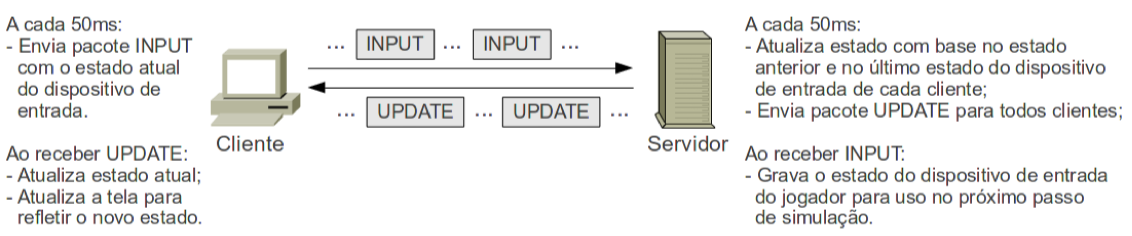
\includegraphics[width=1.03\textwidth]{imagem_81.png}
    \vspace{-20pt}
  \end{figure}
  \begin{itemize}
    \item Custo: O($N^2$)
    \begin{itemize}
      \item maneiras de se mitigar
    \end{itemize}
  \end{itemize}
\end{frame}

% 8.3.2 Filtragem por interesse
\begin{frame} 
  \frametitle{8.3.2 Filtragem por interesse}
  \begin{itemize}
    \item Envio de dados aos avatares relevantes (próximos e visíveis)
    \item Exemplo: mundo virtual simplificado com 4 avatares
  \end{itemize}
  \begin{figure}[h]
    \centering
    \vspace{-18pt}
    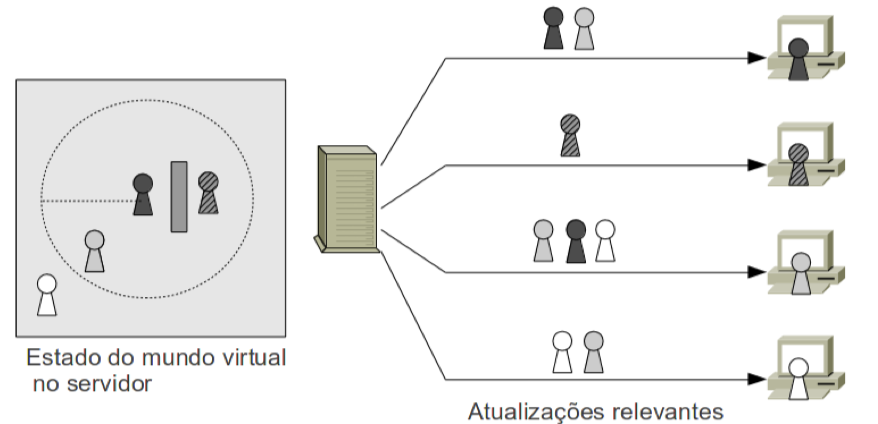
\includegraphics[width=1.03\textwidth]{imagem_82.png}
    \vspace{-20pt}
  \end{figure}
\end{frame}

\begin{frame} 
  \frametitle{8.3.2 Filtragem por interesse: avatares}
  \begin{itemize}
    \item Listrado: atrás da parede e não é relevante os para outros
  \end{itemize}
  \begin{figure}[h]
    \centering
    \vspace{-18pt}
    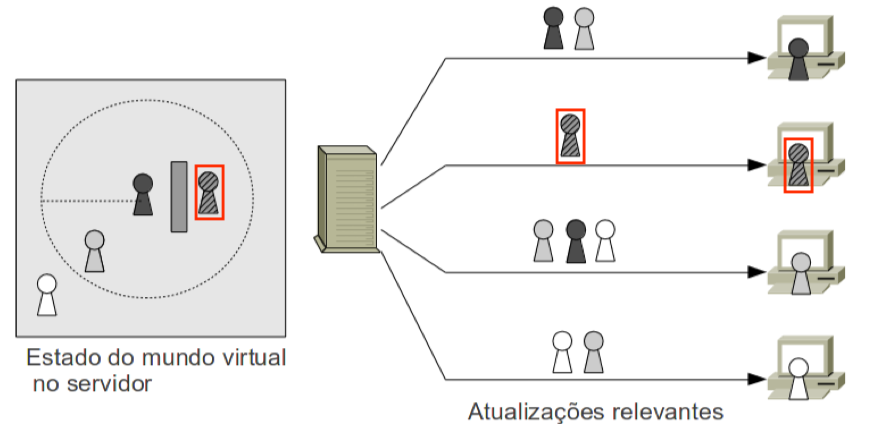
\includegraphics[width=1.03\textwidth]{imagem_82_Listrado.png}
    \vspace{-20pt}
  \end{figure}
\end{frame}

\begin{frame} 
  \frametitle{8.3.2 Filtragem por interesse: avatares}
  \begin{itemize}
    \item Cinza: entre os avatares branco e preto, sendo relevante a eles
  \end{itemize}
  \begin{figure}[h]
    \centering
    \vspace{-18pt}
    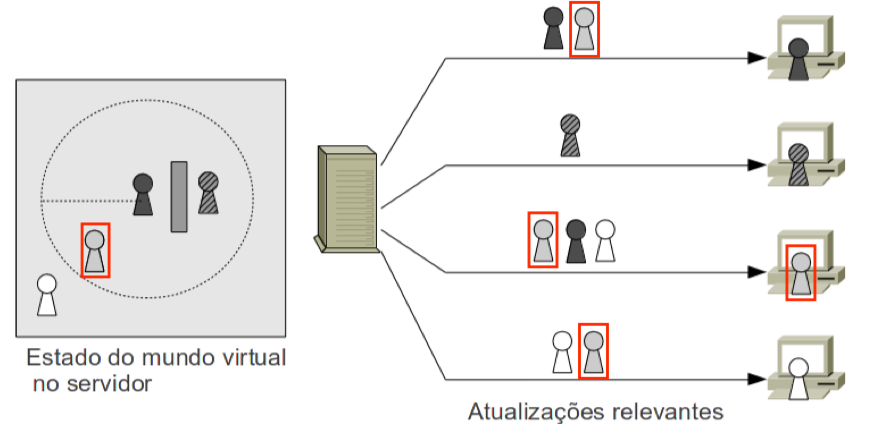
\includegraphics[width=1.03\textwidth]{imagem_82_Cinza.png}
    \vspace{-20pt}
  \end{figure}
\end{frame}

\begin{frame} 
  \frametitle{8.3.2 Filtragem por interesse: avatares}
  \begin{itemize}
    \item Preto: círculo pontilhado - área de interesse
    \item fora da área: irrelevantes (poupando processamento)
  \end{itemize}
  \begin{figure}[h]
    \centering
    \vspace{-18pt}
    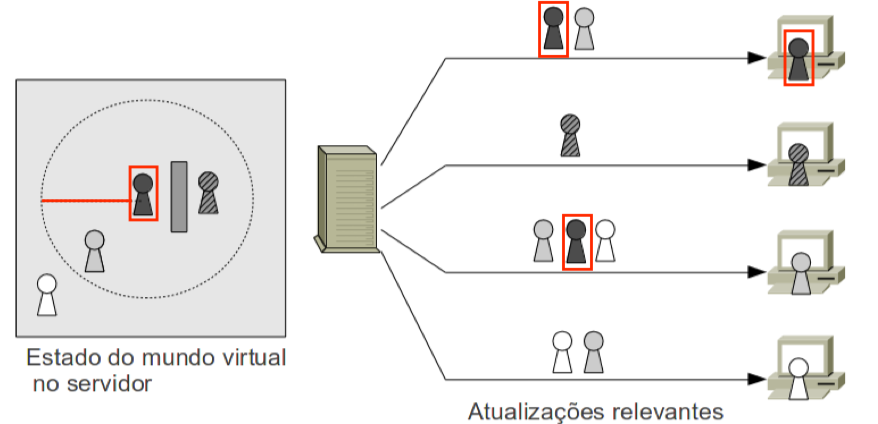
\includegraphics[width=1.03\textwidth]{imagem_82_Preto.png}
    \vspace{-20pt}
  \end{figure}
\end{frame}

\begin{frame}{}
  \frametitle{8.3.2 Filtragem por interesse}
  Priorização por relevância
    \begin{itemize}
      \item Após a Filtragem por Interesse
      \item Largura de banda é limitada
      \begin{itemize}
          \item Servidor: quais atualizações enviar (passo de simulação)
          \item Exemplo: 
          \begin{itemize}
              \item Cercado por $N$ avatares, largura de banda $N/2$ atualizações
              \item Passos pares: primeiros $N/2$ avatares
              \item Passos ímpares: últimos $N/2$ avatares
          \end{itemize}
      \end{itemize}
      \item Reduz-se a qualidade - mantém-se a atualização geral
    \end{itemize}
\end{frame}

% 8.3.3 Extrapolação de movimentos
\begin{frame}
  \frametitle{8.3.3 Extrapolação de movimentos}
  \begin{itemize}
    \item Previsão de posições para suavizar animações
    \item Técnica: Dead-reckoning
    \item Equação balística: último vetor de velocidade recebido para um objeto remoto permanece constante
  \end{itemize}
  \begin{figure}[h]
    \centering
    \vspace{-18pt}
    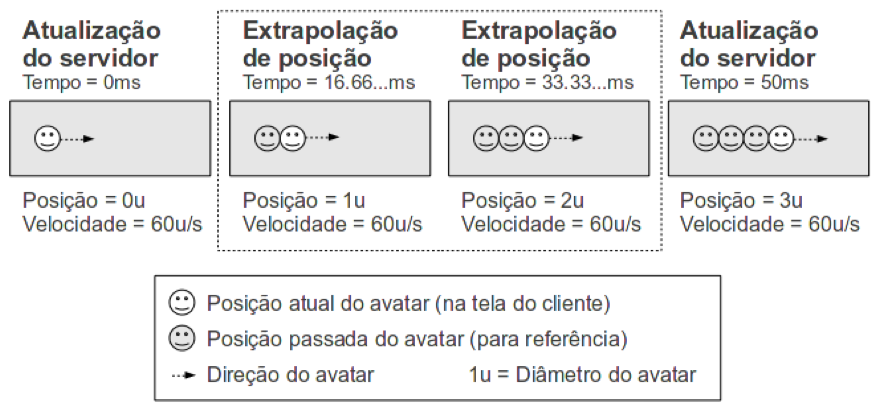
\includegraphics[width=1.03\textwidth]{imagem_83.png}
    \vspace{-20pt}
  \end{figure}
\end{frame}

% 8.3.4 Predição local de movimentos
\begin{frame}
  \frametitle{8.3.4 Predição local de movimentos}
  \begin{itemize}
    \item Resolver problemas da "Extrapolação de movimentos"
    \item Reduz latência percebida pelo usuário
    \item Cliente: precisa simular a aceleração e a animação do avatar
    \item Induz uma complexidade adicional no lado cliente
    \item Jogos online multijogador: usam essas técnicas
    \begin{itemize}
      \item Protocolo
      \item Filtragem por interesse
      \item Extrapolação de movimentos (Dead-reckoning)
      \item Predição local de movimentos
    \end{itemize}
    \item Técnica Heartbeat
    \begin{itemize}
      \item "Batimento Cardíaco" / Pulso de Comunicação
      \begin{flushright}
        \scriptsize
          Eduardo \textit{et al.} (2002)
      \end{flushright}
    \end{itemize}
  \end{itemize}
\end{frame}

\begin{frame}
  \frametitle{Técnica Heartbeat}
  \begin{itemize}
    \item \textbf{Definição}: sinalização periódica entre clientes e servidores
    \item \textbf{Objetivos}:
    \begin{itemize}
      \item Verificar se clientes e servidores estão ativos
      \item Detectar falhas de conexão ou inatividade
      \item Enviar atualizações do estado do servidor para o cliente
    \end{itemize}
    \item \textbf{Funcionamento}:
    \begin{itemize}
      \item Envio de mensagens de "heartbeat" em intervalos regulares
      \item Ausência de heartbeat indica desconexão ou falha
    \end{itemize}
    \item \textbf{Aplicações}:
    \begin{itemize}
      \item Gerenciar sessões de usuários
      \item Liberar recursos de clientes desconectados
      \item Manter a integridade do ambiente virtual
    \end{itemize}
  \end{itemize}
  \begin{flushright}
    \scriptsize
    Eduardo \textit{et al.} (2002)
  \end{flushright}
\end{frame}

\begin{frame}
  \frametitle{Técnica: Dead-reckoning}
  \begin{itemize}
    \item Processo de Atualização do Ambiente Virtual
  \end{itemize}
  \begin{figure}[h]
    \centering
    \vspace{-18pt}
    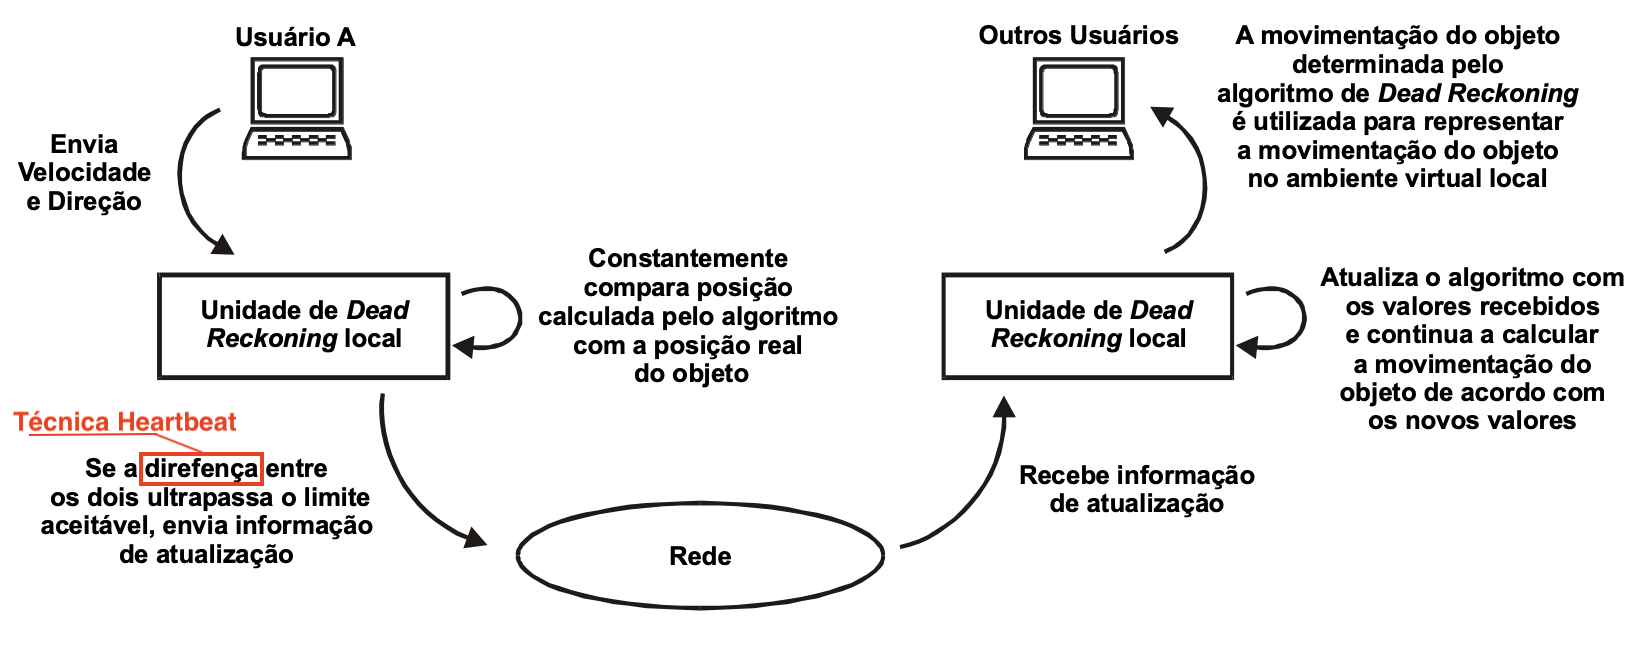
\includegraphics[width=1.03\textwidth]{imagem_Deadreckoning.png}
    \vspace{-20pt}
  \end{figure}
  \begin{flushright}
    \scriptsize
    Eduardo \textit{et al.} (2002)
  \end{flushright}
\end{frame}

\begin{frame}
  \frametitle{Técnica: Dead-reckoning}
  \begin{itemize}
    \item Diferença de Movimento Real e Calculado
  \end{itemize}
  \begin{figure}[h]
    \centering
    \vspace{-18pt}
    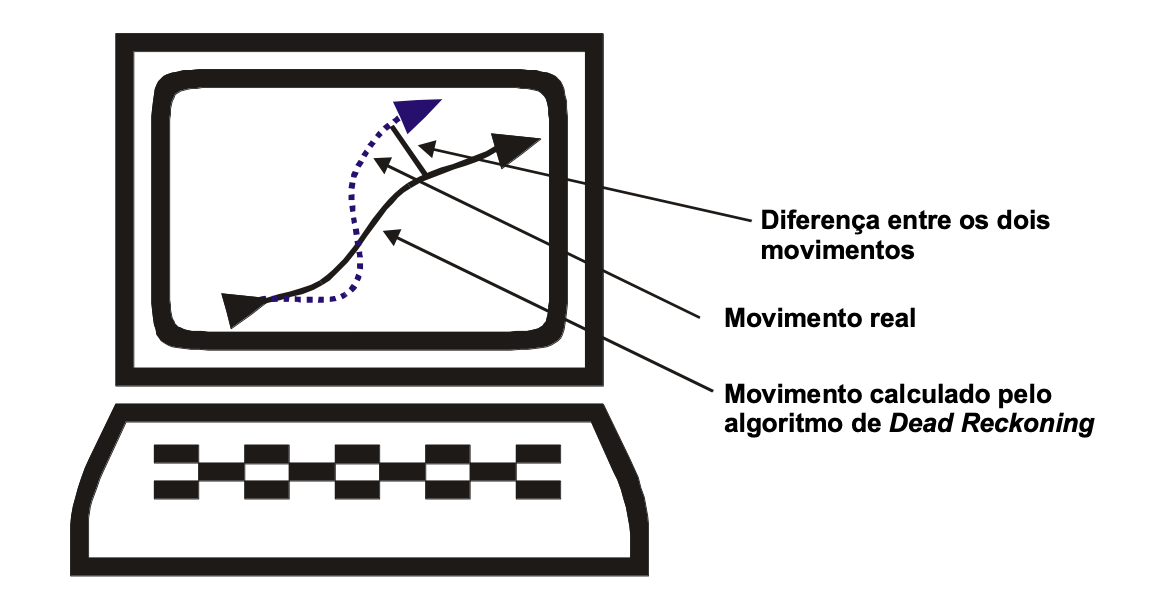
\includegraphics[width=1.03\textwidth]{imagem_DeadreckoningDiferenca.png}
    \vspace{-20pt}
  \end{figure}
  \begin{flushright}
    \scriptsize
    Eduardo \textit{et al.} (2002)
  \end{flushright}
\end{frame}

% \begin{frame}
%   \frametitle{Técnicas usadas}
%   \begin{figure}[h]
%     \centering
%     \vspace{-18pt}
%     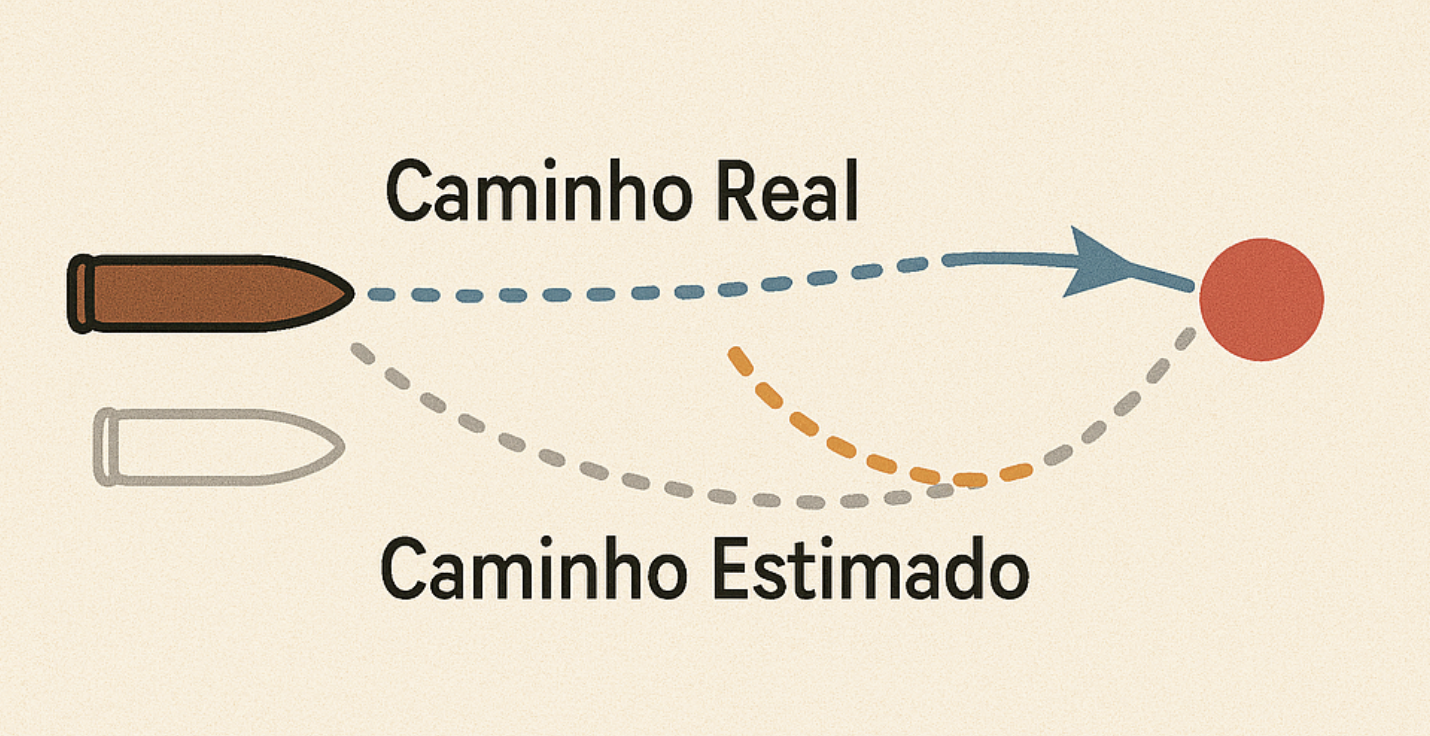
\includegraphics[width=1.03\textwidth]{imagem_83_nova.png}
%     \vspace{-20pt}
%   \end{figure}
% \end{frame}

% 8.4 Sincronização entre servidores de um mesmo AVD
\section{8.4 Entre servidores}

\begin{frame}
  \frametitle{8.4 Sincronização entre servidores}
  \begin{itemize}
    \item Centenas de milhares de usuários simultâneos
    \item Estratégia de distribuir a função de simulação do lado servidor
    \item Rede em múltiplas máquinas servidoras
    \item Algoritmo de simulação distribuída interativa
    \begin{itemize}
      \item Dividir mundo virtual: células contíguas (simulação distribuída)
      \item Reservar processo lógico para cada uma dessas células
      \item Processo lógico fica responsável pela simulação local
      \item Objeto move além da fronteira: transfere processo
      \item Problema: concentrações de objetos interativos
      \begin{itemize}
        \item tráfego de comandos entre células  adjacentes
        \item células adjacentes subutilizadas
      \end{itemize}
    \end{itemize}
  \end{itemize}
\end{frame}

\begin{frame}
  \frametitle{8.4 Sincronização entre servidores}
  \begin{figure}[h]
    \centering
    \vspace{-18pt}
    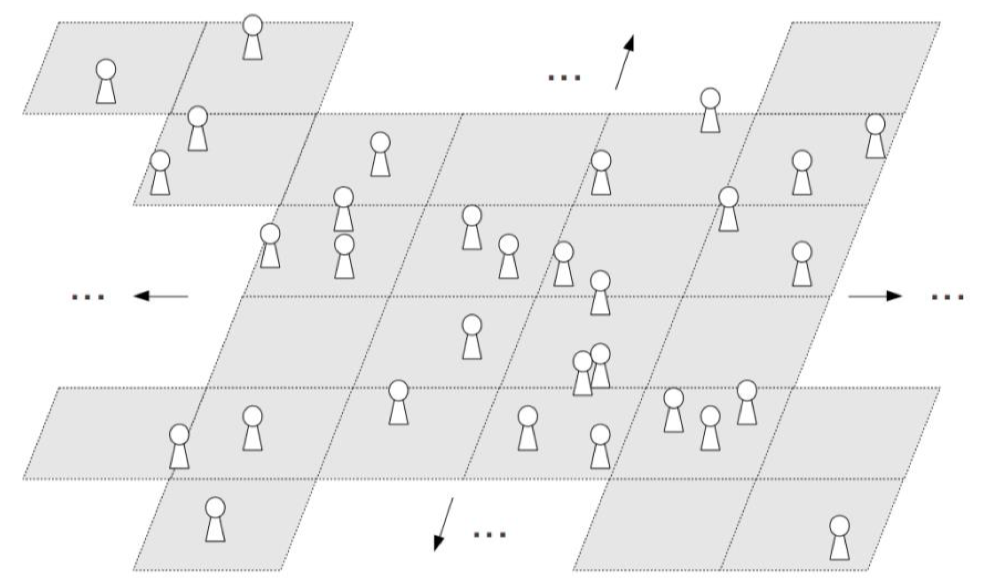
\includegraphics[width=1.03\textwidth]{imagem_84.png}
    \vspace{-20pt}
  \end{figure}
\end{frame}

\begin{frame}
  \frametitle{Perguntas ...}
  XR Distribuído – Técnicas de Sincronização \\
  Ambientes virtuais online (cap 8 até 8.4 - pag. 120 a 129)
  \begin{figure}[h]
    \centering
    \vspace{-18pt}
    
\includegraphics[width=1.03\textwidth]{../qrcode_udesc_trabalho_05.png}
    \vspace{-20pt}
  \end{figure}
\end{frame}

\end{document}
